\documentclass[a4paper]{elsarticle}

\usepackage{amsmath,amssymb}
\usepackage{booktabs}
\usepackage{array}
\usepackage{tabularx}
\usepackage{ragged2e}
\usepackage{tikz}
\usetikzlibrary{arrows.meta,positioning,calc}
\usepackage{graphicx}
\usepackage{hyperref}
\usepackage{geometry}
\geometry{a4paper, margin=1in, columnsep=25pt}
\setlength{\parindent}{0pt}
\setlength{\parskip}{6pt}
\renewcommand{\arraystretch}{1.25}

\journal{Computer Methods and Programs in Biomedicine}

\begin{document}

\onecolumn

{
\setlength{\parskip}{1pt}
\setlength{\parindent}{0pt}
\begin{frontmatter}

\title{Transparent Implementation and Verification of a Medicine Substitution-Scoring Algorithm:\\Deterministic Scoring and Unit-Consistent Dose Handling}

\author[1]{Ajinkya Jiman\footnote{ORCID: 0000-0002-9239-5542}}
\author[1]{Dr.~K.~Rajeswari\footnote{ORCID: 0000-0002-5392-3920}}
\author[1]{Ruturaj Warkad\footnote{ORCID: 0009-0002-5318-9268}}
\author[1]{Vivek Painjane\footnote{ORCID: 0009-0008-4288-1885}}
\author[1]{Yash Mahajan\corref{cor1}\footnote{ORCID: 0009-0004-3789-1641}}
\author[1]{Aryan Wankhade\footnote{ORCID: 0009-0006-3026-8261}}

\affiliation[1]{
  organization={Pimpri Chinchwad College of Engineering},
  addressline={Pune, 411044, Maharashtra},
  country={India}
}

\cortext[cor1]{Corresponding author. Email: yash.mahajan23@pccoepune.org}

\begin{abstract}
\textbf{Background and Objective.} Medicine shortages require pharmacists to rank candidate substitute products by substitutability. Existing medicine-substitution methods are published as specifications without public source code, so an independent implementation cannot be verified. Caviglioli et al. published a degree-of-substitutability (DS) score based on five EDQM Standard Terms, an ATC code, and an NDXUP value, but their implementation is an unreleased Excel macro. Our objective is to implement the published algorithm from its specification alone, verify every publicly labelled result, document discrepancies, and propose a fixed-dose-combination extension clearly labelled as unvalidated.

\textbf{Methods.} We implemented the DS score as a deterministic Python function: each product is encoded as ATC | BDF | AME | ISI | RCA | TRN | NDXUP, candidates sharing the query's ATC are scored, and DS = 100 $-$ (penalty$_\text{NDXUP}$ + penalty$_\text{STs}$). We provide two scoring modes (paper-as-printed and publication-compatible with a documented Table 1 correction), two unit conventions for the fixed-dose-combination NDXUP formula, and a MediGen fixed-dose-combination composite extension labelled as preliminary and unvalidated. Correctness is covered by a 196-assertion test suite.

\textbf{Results.} The implementation reproduces 26/32 published Table 8 DS scores under the paper-as-printed mode; all six failures are parenteral injections off by exactly 1.2152. Under a proposed reconciliation---a transposition of two adjacent Table 1 rows (TRA-0039/TRA-0040) inferred from the published scores---all 32 scores reproduce within rounding (max error 0.0293, ranking identical). Table 7 cannot be reproduced under a single unit convention (unit-aware: 3/5; literal: 4/5). All 196 assertions pass; scoring scales linearly at about 11 microseconds per candidate (90 ms at 8192 candidates).

\textbf{Conclusions.} The implementation independently reproduces the available labelled examples of the published specification under a documented interpretation, with honest documentation of where the published tables are internally inconsistent. The fixed-dose-combination extension is explicitly labelled as our own preliminary adaptation and is unvalidated against published ground truth. No clinical interchangeability or therapeutic-equivalence claim is made. The implementation, test suite, and generated outputs are available at \href{https://github.com/yashmahajan11234567/cmpb-medicine-substitution-scoring}{GitHub repository} (DOI: \href{https://doi.org/10.5281/zenodo.23774017}{10.5281/zenodo.23774017}).
\end{abstract}

\begin{keyword}
medicine substitution; drug shortage; substitutability score; deterministic algorithm; EDQM Standard Terms; fixed-dose combination; reproducibility
\end{keyword}

\end{frontmatter}
}

\twocolumn

\section{Introduction}
\label{sec:intro}

When a branded medicine is temporarily unavailable, pharmacists must shortlist equivalent or alternative products from the market. The shortlist should be ordered by how substitutable each candidate is---not merely by price or availability. This requires a reproducible, evidence-based scoring method that maps structured pharmaceutical attributes to a single comparability score.

Caviglioli et al.\citep{caviglioli2025medicine} published such a method: a \emph{degree of substitutability} (DS) score that encodes each marketed medicinal product on five EDQM Standard Terms (BDF, AME, ISI, RCA, TRN) plus an ATC code and an NDXUP value, then computes a pairwise distance between a lacking product and every alternative \citep{caviglioli2025medicine}. The method is attractive because it is transparent, rule-based, and requires no training data.

However, transparency is not the same as verifiability. Caviglioli's implementation is an unreleased Excel macro; no public source code or dataset accompanies the paper. An independent group cannot re-run the algorithm, confirm its published numbers, or adapt it without re-\\ implementing it from the specification. This gap---a published computational method without a publicly auditable implementation---is the problem this paper addresses.

Our contribution is an independent, deterministic implementation of the published DS algorithm, tested against every labelled result the paper releases. We separate components inherited unchanged from the specification from components we designed, corrected, or extended. We do not claim that the scoring rules are novel: the core algorithm (Standard Term encoding, penalty tables, DS formula, ranking) is Caviglioli et al.'s. What is ours is the implementation, the verification protocol, the proposed reconciliation of table-level inconsistencies, and the fixed-dose-combination extension---each clearly labelled.

The concrete value of this implementation is threefold. First, it makes the published algorithm independently auditable: because the original implementation is an unreleased Excel macro, no external group could previously confirm its published numbers or adapt it to new catalogues. Second, our implementation exposes the full penalty breakdown per candidate (NDXUP penalty, per-term NRD, weighted contributions), which the published macro does not report---this enables pharmacists and researchers to understand *why* a particular candidate receives a particular score, not just what the score is. Third, our two scoring modes and two unit conventions make the specification's ambiguities explicit rather than hidden: the difference between 26/32 and 32/32 matches, and between 3/5 and 4/5 Table 7 rows, is visible and quantifiable rather than silently absorbed.

\section{Related work and research gap}
\label{sec:related}

Computational reproducibility has been recognized as a cornerstone of trustworthy scientific research \citep{nationalacademies2019reproducibility,peng2011reproducible,peng2006reproducible}. The concept originated in computational geophysics, where Claerbout and Karrenbach (1992) argued that an article about computational results is ``advertising, not scholarship''---the actual scholarship is the complete software environment and instructions that generated the figures \citep{claerbout1992electronic}. Buckheit and Donoho (1995) later formalized this idea in the context of wavelet software \citep{buckheit1995wavelab}. Best practices for computational science have since been formalized, emphasizing code and data sharing, computational environment documentation, and workflow transparency \citep{stodden2014reproducible,stodden2014best,wilson2014best,taschuk2017ten,wilson2017good}.

Concerns about the reliability of published research findings are longstanding \citep{ioannidis2005false}. Large-scale replication efforts have shown that many published findings do not reproduce \citep{nosek2015estimating}. Data stewardship principles such as FAIR provide a relevant framing for computational artifacts \citep{wilkinson2016fair}.

Prior work on computational reproducibility in medicine spans author-facing standards, experimental-variability control, and data-processing pipelines \citep{heil2021reproducibility,anderson2013ethical,zhao2020quantify,wagner2022fairly,sandve2013ten}. Our contribution is backward-facing: an independent implementation and verification of one already-published computational method, not a forward-facing standard.

In the specific domain of medicine substitution, Caviglioli et al.\citep{caviglioli2025medicine} is the closest published algorithm to generic-substitution scoring \citep{caviglioli2025medicine}. It encodes products on EDQM Standard Terms and scores pairwise substitutability. Two boundaries must be stated plainly:

\begin{enumerate}
\item The paper is \textbf{single-API}: each product contains one active ingredient. It does \textbf{not} solve one-to-many ingredient reconstruction, and nothing in its method establishes that capability.
\item Fixed-dose combinations (FCs) are \textbf{partially covered, not scored}. The paper supplies a fictitious-ATC rule (Table 6) and an FC NDXUP formula (Equation 4) but never computes a DS score for an FC and never searches over candidate sets of products.
\end{enumerate}

The methodological gap is therefore: an implementation of a published substitution-scoring algorithm that can be independently verified, with documented handling of the specification's internal inconsistencies, and an explicit extension for fixed-dose-combination reconstruction that is honestly labelled as unvalidated.

\section{Method}
\label{sec:method}

\subsection{Product encoding and scoring rule}

Caviglioli et al.\citep{caviglioli2025medicine} encode each medicinal product (MP) as:

\resizebox{\columnwidth}{!}{%
\(\text{ATC} \mid \text{BDF} \mid \text{AME} \mid \text{ISI} \mid \text{RCA} \mid \text{TRN} \mid \text{NDXUP}\)%
}

where ATC is the Anatomical Therapeutic Chemical code \citep{who2026atcddd}; BDF/AME/ISI/RCA/TRN are EDQM Standard Terms with a relative position (RP) inside each ordered scale \citep{edqm2024standard,iso202311239}; and NDXUP is the number of defined daily doses per presentation unit \citep{who2026atcddd}.

The DS score of a lacking product (\emph{lak}) against a candidate (\emph{sub}) sharing its ATC code is:

\begin{equation}
\text{DS} = 100 - (\text{penalty}_{\text{NDXUP}} + \text{penalty}_{\text{STs}})
\label{eq:ds}
\end{equation}

where:

\begin{equation}
\text{penalty}_{\text{NDXUP}} \in \{0,2,4,6,8,10\}
\label{eq:ndxup}
\end{equation}
\text{from Table 4 of the specification}

\begin{equation}
\begin{gathered}
\text{penalty}_{\text{STs}} = \sum_{\text{st}\in\{\text{BDF,AME,ISI,RCA,TRN}\}} \\
\text{NRD}_{\text{st}} \cdot w_{\text{st}} \cdot \frac{80}{100}
\end{gathered}
\label{eq:st}
\end{equation}

\begin{equation}
\text{NRD}_{\text{st}} = \frac{|\text{RP}_{\text{lak}} - \text{RP}_{\text{sub}}|}{\max\text{difference}_{\text{st}}} \times 100
\label{eq:nrd}
\end{equation}

where
\begin{equation*}
\begin{gathered}
w = (\text{BDF }0.46,\ \text{AME }0.18,\ \text{ISI }0.20,\\
\phantom{w = (}\text{RCA }0.09,\ \text{TRN }0.07)
\end{gathered}
\end{equation*}
(Table 5 of the specification).
Products whose entire code string matches the query are pharmaceutical equivalents (DS = 100); everything else with the same ATC is an alternative, ranked by decreasing DS.

\begin{figure}[htbp]
\centering
\resizebox{\columnwidth}{!}{%
% Figure 1: DS score decomposition
% Clean, minimal TikZ diagram showing DS = 100 - (penalty_NDXUP + penalty_STs)
% with the five EDQM Standard Terms branching from penalty_STs

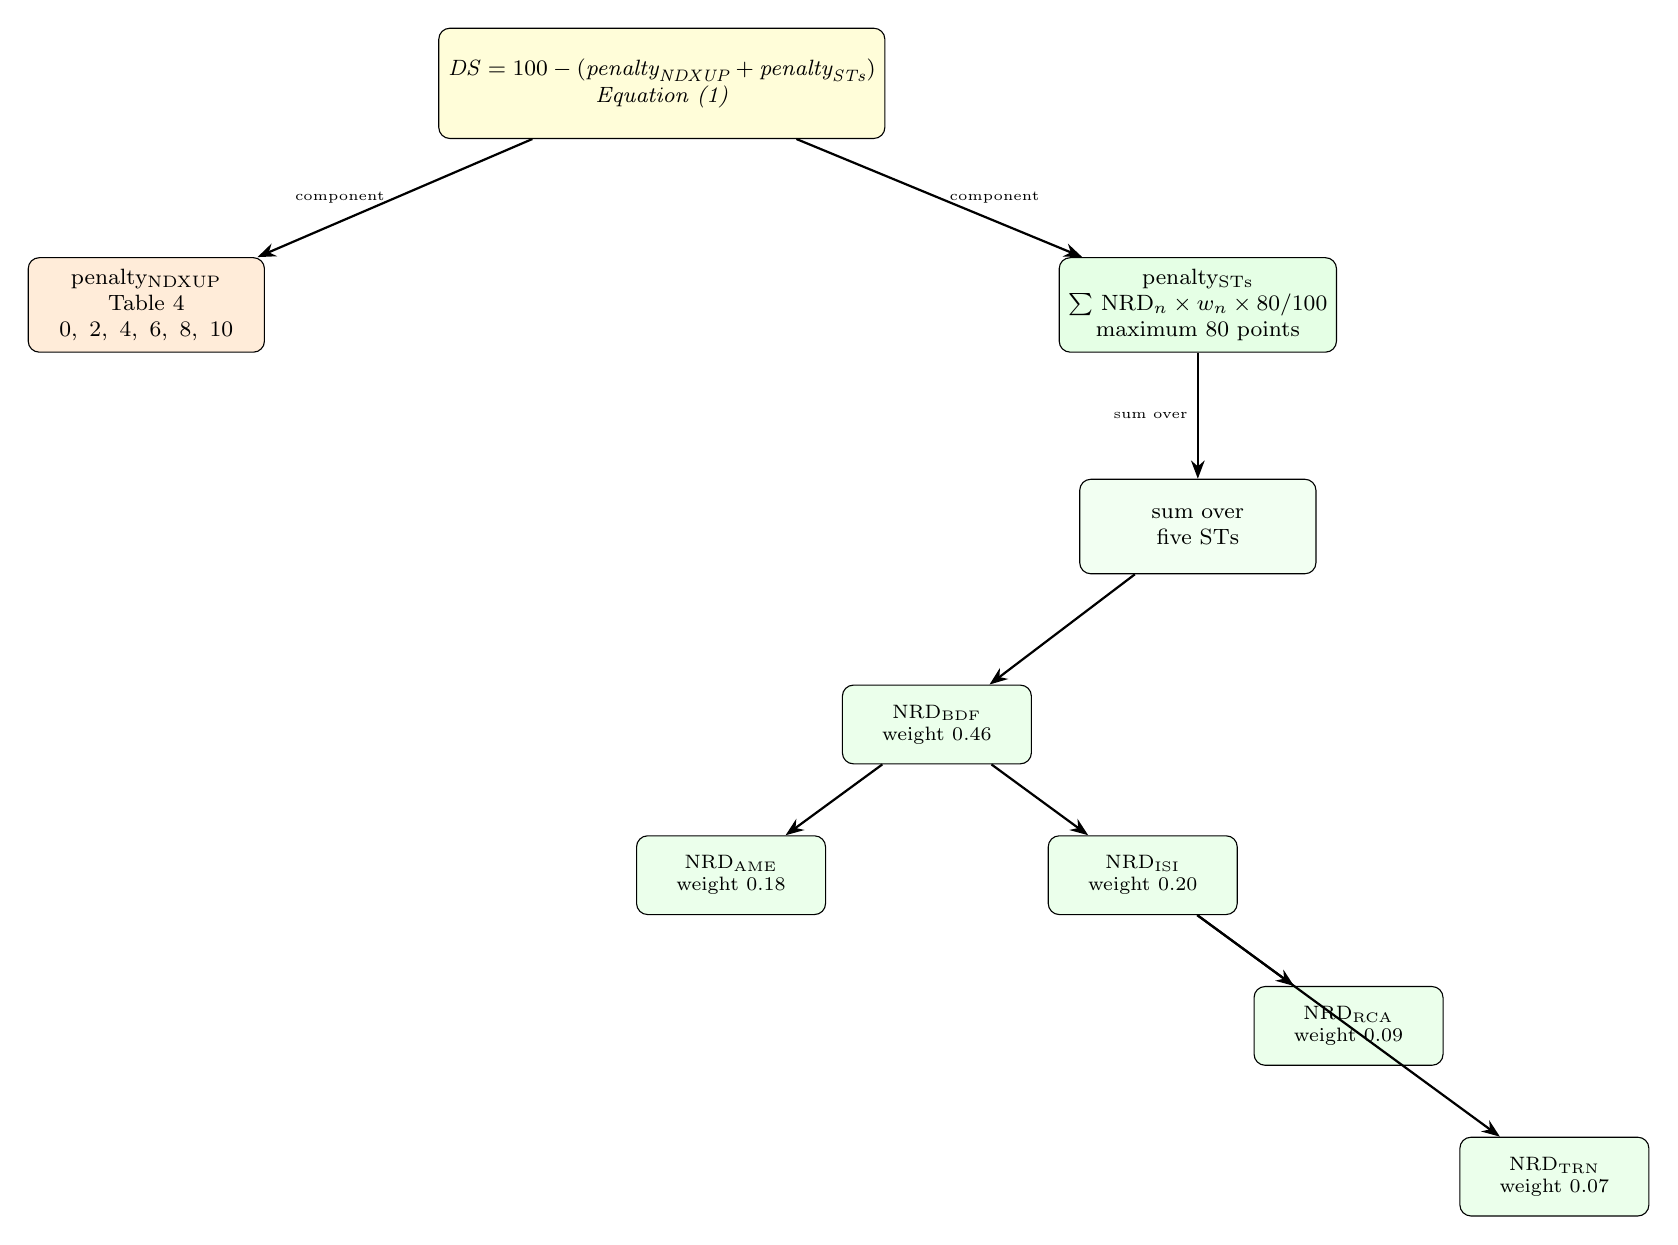
\begin{tikzpicture}[
    node distance = 1.5cm and 2.2cm,
    root/.style = {draw, rounded corners, align=center, minimum width=4.4cm, minimum height=1.4cm, font=\footnotesize\itshape, fill=yellow!15},
    comp/.style = {draw, rounded corners, align=center, minimum width=3.0cm, minimum height=1.2cm, font=\footnotesize, fill=blue!10},
    leaf/.style = {draw, rounded corners, align=center, minimum width=2.4cm, minimum height=1.0cm, font=\scriptsize, fill=green!8},
    arrow/.style = {-Stealth, thick},
    edge/.style = {font=\scriptsize, align=center, text width=1.6cm},
]

% Root: DS formula
\node[root] (ds) {DS $= 100 - (\text{penalty}_{\text{NDXUP}} + \text{penalty}_{\text{STs}})$\\ Equation (1)};

% Left branch: penalty_NDXUP
\node[comp, fill=orange!15, below left=of ds] (p1) {penalty$_{\text{NDXUP}}$\\ Table 4\\ $0,\ 2,\ 4,\ 6,\ 8,\ 10$};

% Right branch: penalty_STs
\node[comp, fill=green!10, below right=of ds] (p2) {penalty$_{\text{STs}}$\\ $\sum\, \text{NRD}_n \times w_n \times 80/100$\\ maximum 80 points};

% Sum over node
\node[comp, fill=green!5, below=1.6cm of p2] (psum) {sum over\\ five STs};

% Individual NRD boxes - arranged in an arc below psum
\node[leaf, below left=1.4cm and 0.6cm of psum] (nrd1) {NRD$_{\text{BDF}}$\\ weight 0.46};
\node[leaf, below left=0.9cm and 0.2cm of nrd1] (nrd2) {NRD$_{\text{AME}}$\\ weight 0.18};
\node[leaf, below right=0.9cm and 0.2cm of nrd1] (nrd3) {NRD$_{\text{ISI}}$\\ weight 0.20};
\node[leaf, below right=0.9cm and 0.2cm of nrd3] (nrd4) {NRD$_{\text{RCA}}$\\ weight 0.09};
\node[leaf, below right=0.9cm and 0.2cm of nrd4] (nrd5) {NRD$_{\text{TRN}}$\\ weight 0.07};

% Arrows from root
\draw[arrow] (ds) -- (p1) node[midway, left, font=\tiny] {component};
\draw[arrow] (ds) -- (p2) node[midway, right, font=\tiny] {component};

% Arrow from p2 to psum
\draw[arrow] (p2) -- (psum) node[midway, left, font=\tiny] {sum over};

% Arrows from psum to individual NRDs
\draw[arrow] (psum) -- (nrd1) node[midway, left, font=\tiny] {};
\draw[arrow] (nrd1) -- (nrd2) node[midway, left, font=\tiny] {};
\draw[arrow] (nrd1) -- (nrd3) node[midway, right, font=\tiny] {};
\draw[arrow] (nrd3) -- (nrd4) node[midway, left, font=\tiny] {};
\draw[arrow] (nrd3) -- (nrd5) node[midway, right, font=\tiny] {};

\end{tikzpicture}%
}
\caption{Decomposition of the DS score into its two penalty components: the NDXUP penalty (Table 4) and the weighted sum of normalised relative distances across the five EDQM Standard Terms. The equation and figure are consistent: DS = 100 $-$ (penalty$_{\text{NDXUP}}$ + penalty$_{\text{STs}}$).}
\label{fig:ds-formula}
\end{figure}

\subsection{Scoring modes: inherited specification and proposed reconciliation}

The specification defines a single interpretation of its tables. We implement two modes:

\begin{itemize}
\item \textbf{V0-strict-baseline:} the specification exactly as printed (Table 1 relative positions, unit-aware Equation 4). This is the faithful reproduction.
\item \textbf{V1-publication-compatible:} V0 with one proposed reconciliation---a transposition of the adjacent Table 1 rows TRA-0039 (Dispersion, RP~7) and TRA-0040 (Dissolution, RP~5), inferred from the published scores, which restores ascending EDQM code order inside the transformation group and reproduces all 32 published Table 8 DS scores.
\end{itemize}

The transposition is inferred from the published scores: it restores ascending EDQM code order inside the transformation group. No other scale, weight, penalty, or parameter is altered. Both modes are reported side by side; neither silently fits parameters.

\subsection{Fixed-dose-combination handling}

Fixed-dose combinations receive two provisions: a fictitious ATC code when the official code is ambiguous (Table 6 of the specification), and an FC NDXUP computed as the sum of per-API dosage/DDD ratios (Equation 4) \citep{fda2006fixed,ema2010fixed,who2005fixed}:

\begin{equation}
\text{NDXUP}_{\text{FC}} = \sum_i \frac{\text{dosage}_i}{\text{DDD}_i}
\label{eq:fc}
\end{equation}

Equation 4 defines NDXUP as the sum of per-API dosage/DDD ratios, but the published Table 7 does not state a single unit convention for the printed quantities. We implement two conventions: a literal convention that divides the printed numbers as they appear, and a unit-normalized convention that converts all quantities to milligrams where the units are compatible. Both conventions are implemented and reported side by side (Section \ref{sec:results-table7}). Numerical matches under either convention do not establish the intended interpretation of the printed quantities: row B's tablet-count DDD cannot be interpreted as a mass ratio without additional information, and row E's literal match reproduces 45 numerically~while mixing mg numerators with g denominators without conversion.

\subsection{V3: MediGen fixed-dose-combination composite extension}
\label{sec:v3}

The specification scores single-API substitution only. For fixed-dose-combination reconstruction we define a composite that keeps the per-API DS as the substitutability signal and adds two provisions the specification lacks:

\begin{enumerate}
\item A \textbf{hard API-coverage requirement}: a candidate set qualifies only when the union of its APIs covers every API of the query.
\item An \textbf{NDXUP distance factor} \linebreak[4]\mbox{$1 - \text{penalty}_{\hbox{NDXUP}}/10$} applied to the reconstructed combination.
\end{enumerate}

The composite is $\text{DS} \times \text{coverage}$ \\
$\times \text{NDXUP factor}$.

This is \textbf{our adaptation}, not a reproduction of any published result: the specification publishes no FC DS score and no candidate-set search, so there is no published ground truth for V3 to be scored against. V3 is implemented and executed on the published catalogue, but no accuracy claim is made. Ingredient and attribute similarity does not establish substitutability; pharmaceutical attributes the encoding omits (strength, pharmacokinetics, excipients, release profile, therapeutic equivalence) are not modelled. No clinical interchangeability is claimed.

\section{Implementation}
\label{sec:implementation}

We implemented the algorithm in Python (3.14) with no hard-coded results: every score is derived from the published scales, weights, and penalty table. The implementation is contained in \texttt{code/}\allowbreak\texttt{ds\_algorithm.py} and provides:

\begin{itemize}
\item The five EDQM Standard Term scales with relative positions (inherited from Table 1 of the specification).
\item The ST weight factors (inherited from Table 5 of the specification).
\item The NDXUP penalty ladder (inherited from Table 4 of the specification).
\item Two scoring modes (V0 strict, V1 publication-compatible) as described in Section \ref{sec:method}.
\item \texttt{ds\_components()} returns the full breakdown: DS, NDXUP penalty, ST penalty per term, NRD values, weighted contributions, and equivalence flag.
\item {\sloppy The function \mbox{\texttt{find\_substitutes}()} returns all catalogue products sharing the query's ATC, ranked by decreasing DS, with pharmaceutical equivalents first. Ties are broken by AIC for a deterministic order.}
\item \texttt{fc\_ndxup\_units()} computes Equation 4 under two unit conventions (unit-aware and literal).
\item \texttt{fictitious\_fc\_atc()} generates fictitious FC ATC codes per Table 6 of the specification.
\item \texttt{validation\_indicators()} computes the ten similarity indicators described in the specification.
\end{itemize}

Invalid and ambiguous records: ST-IDs not present in a scale raise \texttt{KeyError}; NDXUP values outside Table 4's branches fall to the maximum penalty of 10; products without a matching ATC are excluded; \mbox{\texttt{find\_substitutes()}} omits them.

The correctness of the implementation is covered by \texttt{code/test\_caviglioli.py}, a 196-assertion suite (Section \ref{sec:tests}).

\begin{figure}[htbp]
\centering
\resizebox{\columnwidth}{!}{%
% Figure 2: Scoring workflow of the implemented method
% Clean, minimal TikZ diagram: query + catalogue -> ATC filter -> DS computation -> ranking -> output

\begin{tikzpicture}[
    node distance = 2.6cm and 3.6cm,
    io/.style = {draw, rounded corners, align=center, text width=3.8cm, minimum height=1.8cm, font=\footnotesize, fill=yellow!15},
    stepbox/.style = {draw, rounded corners, align=center, text width=3.6cm, minimum height=2.0cm, font=\footnotesize, fill=blue!8},
    arrow/.style = {-Stealth, thick},
]

% Left: inputs
\node[io] (input) {Query product\\ ATC + ST codes + NDXUP\\ Catalogue of candidates};

\node[stepbox, right=of input] (s1) {1. ATC filter\\ keep candidates sharing query ATC};

\node[stepbox, right=of s1] (s2) {2. DS computation\\ per candidate\\ Eqs.~(1)--(4)};

\node[stepbox, right=of s2] (s3) {3. Ranking\\ equivalents first\\ then descending DS};

\node[io, right=of s3] (output) {Ranked substitute list\\ with DS scores\\ and penalty breakdown};

% Forward arrows
\draw[arrow] (input) -- (s1) node[midway, above, font=\scriptsize] {input attributes};
\draw[arrow] (s1) -- (s2) node[midway, above, font=\scriptsize] {filtered candidates};
\draw[arrow] (s2) -- (s3) node[midway, above, font=\scriptsize] {DS per candidate};
\draw[arrow] (s3) -- (output) node[midway, above, font=\scriptsize] {ranked output};

% Add extra space at top for LaTeX caption clearance
\path (current bounding box.north) -- ++(0,0.8cm);

\end{tikzpicture}%
}
\caption{Scoring workflow of the implemented method: query product and catalogue are filtered by ATC, each candidate is scored with Equations~(1)--(4), results are ranked with equivalents first, and the ranked substitute list is produced.}
\label{fig:workflow}
\end{figure}

\section{Experimental design and evaluation protocol}
\label{sec:experiment}

\subsection{Dataset}
\label{sec:data}

The only labelled public artefact from the specification is Table 8: 32 risperidone products (AIC, EDQM ST codes, NDXUP) with a published DS score for each, computed against the query risperidone~2~mg film tablet (AIC 037599230). The paper's own validation-indicator percentages were computed on a proprietary test set (Farmadati Italia + AIFA shortage list) that was not released \citep{caviglioli2025medicine}; those percentages therefore cannot be recomputed. Table 8 is the sole labelled data we score against.

Table 7 supplies five illustrative fixed-dose combinations with published NDXUP sums, used to test Equation 4 under two unit conventions.

\subsection{Evaluation criteria}
\label{sec:criteria}

A reproduced DS score counts as a match when it agrees with the published value within the published rounding (one decimal place, tolerance 0.05). We also report mean absolute error (MAE), maximum absolute error, Kendall tau against the published ranking order, and top-1 agreement.

For Table 7, a reproduced NDXUP sum counts as a match under tolerance 0.005.

\subsection{Reproducibility}
\label{sec:repro}

The implementation, datasets, and all generated outputs are contained in the project directory. Every number in this manuscript is traceable to the JSON artefacts produced by the code. Runtime and memory were measured on a synthetic catalogue (32--8192 candidates) used for scaling only; no accuracy is claimed from it.

\section{Results}
\label{sec:results}

\subsection{Worked example}
\label{sec:results-worked}

The specification's worked example computes the normalised relative distance (NRD) between a tablet and a syrup on the BDF scale, reporting NRD = 41.30 and a weighted contribution of $41.30 \times 0.46 = 18.998$. Our implementation reproduces these values within the published precision: NRD 41.3043 (published 41.30; absolute error 0.0043) and weighted contribution 19.0000 (published 18.998; absolute error 0.0020).

\subsection{Table 8: DS scores against the published table}
\label{sec:results-table8}

\begin{table}[htbp]
\centering\small
\caption{Reproduction of the 32 published Table 8 DS scores under two scoring modes. Match tolerance: 0.05 (published one-decimal rounding).}
\label{tab:table8}
\resizebox{\columnwidth}{!}{%
\begin{tabular}{@{}lccc@{}}
\toprule
Mode & Matches / 32 & MAE & Max abs error \\
\midrule
V0-strict-baseline (specification as printed) & 26 & 0.2290 & 1.2152 \\
V1-publication-compatible (proposed reconciliation) & 32 & 0.0066 & 0.0293 \\
\bottomrule
\end{tabular}%
}
\end{table}

Table \ref{tab:table8} summarises the outcome. Under V0, all six failures are parenteral injections (IM products), each off by exactly 1.2152. The mismatch is isolated to the TRN scale: the published values require the six parenteral products at relative position 5, while the printed Table 1 places them at position 7.

Under V1---which applies the proposed reconciliation of the adjacent Table 1 rows TRA-0039 and TRA-0040---all 32 published DS scores reproduce within tolerance (MAE 0.0066, max error 0.0293), and the published ranking order is identical (Kendall tau 1.0). The reconciliation is inferred from the published scores: no other scale, weight, penalty, or parameter is altered.

\subsection{Table 4: NDXUP penalty ladder}
\label{sec:results-table4}

All 7 branches of the Table 4 penalty ladder reproduce exactly: equal NDXUP $\to$ 0, half $\to$ 2, double $\to$ 4, between $0.5\times$ and $1\times$ $\to$ 6, between $1\times$ and $2\times$ $\to$ 8, below half $\to$ 10, above double $\to$ 10.

\subsection{Table 6: fictitious-ATC rule}
\label{sec:results-table6}

The stated rule---keep the fourth ATC level of the API with the main therapeutic effect and assign an unused fifth level from 99 down to 80---is satisfied for every row (5/5). However, the authors' actual digits (95, 96) are not the highest free value (99). The constraint holds; the specific allocation order is not recoverable from the paper.

\subsection{Table 7: fixed-dose-combination\\ NDXUP sums}
\label{sec:results-table7}

\begin{table}[htbp]
\centering\small
\caption{Reproduction of the 5 published Table 7 NDXUP sums under two unit conventions. A row counts as reproduced when \emph{some} convention matches.}
\label{tab:table7}
\resizebox{\columnwidth}{!}{%
\begin{tabular}{@{}p{4.2cm}cc@{}}
\toprule
Convention & Matches / 5 & Notes \\
\midrule
Unit-aware (convert all quantities to mg) & 3 & Row C (3~g DDD) needs conversion \\
Literal (divide printed numbers) & 4 & Rows B and E need the literal division \\
Any convention & 5 & Every row reproducible by at least one \\
\bottomrule
\end{tabular}%
}
\end{table}

No single convention reproduces all five published Table 7 NDXUP sums: the unit-normalized calculation reproduces 3 of 5 (rows A, C, D) and the literal calculation reproduces 4 of 5 (rows A, B, D, E). Every row matches under at least one convention. However, numerical agreement under a convention does not establish that convention as the intended interpretation of the printed quantities: row B's tablet-count DDD cannot be interpreted as a mass ratio without additional information, and row E's literal calculation reproduces 45 numerically~while mixing mg numerators with g denominators without conversion.

A numerical match under the literal convention is not evidence of dimensional correctness. Table~\ref{tab:table7-dim} shows the dimensional analysis for each row: the literal convention treats the printed DDD as a bare number (so for gentamycin the combined literal calculation is 30/1 + 30/2 = 45, matching the published total numerically; the individual gentamycin contribution is 30/1 = 30, not 45,~while mixing mass units without conversion), while the unit-aware convention converts all quantities to milligrams before division (gentamycin: 30~mg/1000~mg~+~30~mg/2000~mg~=~0.045, not matching the published 45). Row B's tablet-count DDD (``1 tab'') cannot be converted to mass and must be treated as a bare count under either convention.

\begin{table}[htbp]
\centering\small
\caption{Dimensional analysis of the 5 published Table 7 NDXUP sums. Dim.\ valid indicates whether the calculation respects unit compatibility (dosage and DDD expressed in compatible units before division). Literal calculation divides printed numbers as they appear; unit-normalized calculation converts all quantities to milligrams where the units are compatible.}
\label{tab:table7-dim}
\resizebox{\columnwidth}{!}{%
\begin{tabular}{@{}p{2.2cm}p{2.6cm}p{3.0cm}p{3.0cm}p{1.5cm}p{1.8cm}@{}}
\toprule
FC example & Printed inputs and units & Literal calculation & Unit-normalized calculation & Published & Dim.\ valid? \\
\midrule
A: Rosuvastatin 10~mg + Ezetimibe 10~mg & 10~mg/10~mg + 10~mg/10~mg & $10/10 + 10/10 = 2.00$ & $10/10 + 10/10 = 2.00$ & 2.00 & Yes \\
B: Desogestrel 0.15~mg + EE 0.03~mg & 0.15~mg/1~tab + 0.03~mg/25~mcg & $0.15/1 + 0.03/25 = 0.1512$ & $0.15/1 + 0.03/0.025 = 1.3500$ & 0.15 & No (tab count) \\
C: Scopolamine 10~mg + Paracetamol 800~mg & 10~mg/60~mg + 800~mg/3~g & $10/60 + 800/3 = 266.8333$ & $10/60 + 800/3000 = 0.4333$ & 0.43 & No (g not converted) \\
D: Amitriptyline 12.5~mg + Chlordiazepoxide 5~mg & 12.5~mg/75~mg + 5~mg/30~mg & $12.5/75 + 5/30 = 0.3333$ & $12.5/75 + 5/30 = 0.3333$ & 0.33 & Yes \\
E: Gentamycin 30~mg + Betamethasone 30~mg & 30~mg/1~g + 30~mg/2~g & $30/1 + 30/2 = 45.00$ & $30/1000 + 30/2000 = 0.0450$ & 45.0 & No (g not converted) \\
\bottomrule
\end{tabular}%
}
\end{table}

Both conventions are implemented and reported side by side rather than one being chosen silently.

\subsection{Variants V0--V3}
\label{sec:results-variants}

\begin{table}[htbp]
\centering\small
\caption{Variant summary. V3 is our MediGen fixed-dose-combination composite extension; it is not evaluated against published ground truth because the specification publishes no FC DS score.}
\label{tab:variants}
\resizebox{\columnwidth}{!}{%
\begin{tabular}{@{}lp{6.2cm}@{}}
\toprule
Variant & Description \\
\midrule
V0-strict-baseline & Specification exactly as printed; 26/32 Table 8 scores match \\
V1-publication-compatible & V0 + proposed Table 1 TRN reconciliation; 32/32 match \\
V2-unit-literal-fc & V1 + literal Equation 4 division; Table 7: 4/5 literal \\
V3-medi-gen-fc-composite & Our FC composite: per-API DS gated by hard API-coverage and an NDXUP factor; not evaluated against published ground truth \\
\bottomrule
\end{tabular}%
}
\end{table}

Table \ref{tab:variants} lists all four variants. V1 and V2 both reproduce all 32 Table 8 scores. V3 (Section \ref{sec:v3}) is our adaptation for fixed-dose-combination reconstruction.

\subsection{Performance scaling}
\label{sec:results-scaling}

Scoring is $O(n)$ in catalogue size with constant work per candidate (five Standard Terms, no learning). On a synthetic catalogue:

\begin{table}[htbp]
\centering\small
\caption{Runtime and memory scaling of the scoring algorithm. Synthetic catalogue; no accuracy claimed.}
\label{tab:scaling}
\resizebox{\columnwidth}{!}{%
\begin{tabular}{@{}lrrrr@{}}
\toprule
Catalogue size & Runtime (ms) & Peak memory (KiB) & $\mu$s per candidate \\
\midrule
32 & 0.57 & 6.3 & 18.56 \\
128 & 1.08 & 23.6 & 8.53 \\
512 & 5.00 & 106.6 & 9.78 \\
2048 & 21.58 & 435.6 & 10.54 \\
8192 & 89.22 & 2163.5 & 10.89 \\
\bottomrule
\end{tabular}%
}
\end{table}

At 8192 candidates, a full pass takes about 90~ms and about 2.1~MiB.

\subsection{Correctness tests}
\label{sec:tests}

The test suite \texttt{code/test\_caviglioli.py} covers the worked example, the Table 4 ladder branch by branch, NRD symmetry and full-span behaviour on every scale, the Table 6 fictitious-ATC rule including the 99--80 exhaustion fallback, Equation 4 under both unit conventions, all 32 Table 8 DS scores per product in both modes, the published ranking order, scoring-mode semantics, DS/component-breakdown consistency and ordering by \mbox{\texttt{find\_substitutes()}}. All 196 assertions pass. Verification and validation testing of research software follows established practices for checking that an implementation correctly reproduces its specification \citep{taschuk2017ten,wilson2017good,stodden2014best}.

\section{Discussion}
\label{sec:discussion}

\subsection{What the verification establishes}
\label{sec:discussion-verification}

The implementation deterministically reproduces the available labelled examples under the documented interpretation: 32/32 Table 8 scores under V1, ranking order identical, all 196 tests passing. But the published document contains a genuine internal inconsistency---the transposed TRN rows in Table 1---and the Table 7 examples yield different numerical matches under different unit conventions (3 of 5 unit-normalized, 4 of 5 literal), with the intended interpretation of the printed quantities not conclusively established. The proposed TRN reconciliation matches the published Table 8 scores, but the underlying table transposition has not been independently confirmed against an authoritative source.

These inconsistencies matter because substitution scoring can influence which product reaches a patient during a shortage. An undetected table error or unit-convention mix-up could propagate silently. Our verification shows where the specification and its own labelled data agree and where they do not.

\subsection{Comparison with prior work}
\label{sec:discussion-comparison}

Caviglioli et al.\citep{caviglioli2025medicine} is the closest published algorithm to generic-substitution scoring, and its EDQM Standard Terms encoding is a useful prior for a reconstruction pipeline. However, it is single-API only and does not address one-to-many ingredient reconstruction. Our V3 extension targets exactly that gap, but it is an unvalidated adaptation---not a claim of clinical superiority.

\subsection{What we do not claim}
\label{sec:discussion-limits}

We do not claim that the algorithm predicts actual substitution outcomes in a pharmacy. The only labelled data is 32 products of one API (risperidone). We do not claim clinical interchangeability, patient safety, or therapeutic equivalence. We do not claim that V3 outperforms any published method---no such comparison is possible from the published data. We do not claim the scoring rules are novel: the core algorithm is inherited from Caviglioli et al.\citep{caviglioli2025medicine}.

\section{Limitations and threats to validity}
\label{sec:limitations}

\begin{enumerate}
\item \textbf{Single labelled dataset.} Only Table 8 (32 risperidone products) is publicly labelled. The paper's own test set (Farmadati Italia + AIFA shortage list) is proprietary and unreleased; its validation-indicator percentages cannot be recomputed.
\item \textbf{One API.} All labelled products contain risperidone. Results may not generalise to other APIs or therapeutic areas.
\item \textbf{Single-API scope.} The specification does not address one-to-many ingredient reconstruction; V3 is our adaptation and is unvalidated.
\item \textbf{No clinical validation.} Nothing here establishes that the algorithm predicts real-world substitution outcomes.
\item \textbf{EDQM scale source.} Our reconciliation of the TRN transposition is inferred from published DS values and the EDQM code order; we could not obtain the authoritative EDQM Standard Terms document itself.
\end{enumerate}

\section{Conclusion}
\label{sec:conclusion}

We implemented Caviglioli et al.\citep{caviglioli2025medicine}'s medicine \linebreak[4]\mbox{substitution-scoring} algorithm from its published description alone, as a deterministic Python implementation. The algorithm is substantially reproducible: under a proposed reconciliation (TRN row transposition inferred from published scores), all 32 published Table 8 DS scores reproduce within tolerance with the ranking order identical. The Table 7 examples yield numerical matches under two different unit conventions (3 of 5 unit-normalized, 4 of 5 literal), but no single convention reproduces all five sums and the intended interpretation of the printed quantities is not established. All 196 correctness assertions pass, and scoring scales linearly (about 11 microseconds per candidate).

{\sloppy The core scoring rules are inherited from Caviglioli et al.\citep{caviglioli2025medicine}; our contributions are the implementation, the verification protocol, the proposed reconciliation of table-level inconsistencies, and the fixed-dose-combination extension---each clearly labelled. The V3 extension is unvalidated against published ground truth. We make no claim of clinical interchangeability or therapeutic equivalence. The implementation, test suite, and generated outputs are available at \href{https://github.com/yashmahajan11234567/cmpb-medicine-substitution-scoring}{GitHub repository} (DOI: \href{https://doi.org/10.5281/zenodo.23774017}{10.5281/zenodo.23774017}).}

\section{Declarations}

\subsection{Ethics statement}
Not applicable---this work uses only published, de-identified product data and synthetic catalogues; no human-subjects research and no patient data were involved.

\subsection{Funding}
This research did not receive any specific grant from funding agencies in the public, commercial, or not-for-profit sectors.

\subsection{Competing interests}
The authors declare that they have no known competing financial interests or personal relationships that could have appeared to influence the work reported in this paper.

\subsection{Author contributions (CRediT)}
Ajinkya Jiman and Dr.\\ K.\\ Rajeswari: mentorship, research guidance.
Ruturaj Warkad, Vivek Painjane, Yash Mahajan, Aryan Wankhade: algorithm implementation, reproduction, discrepancy analysis, benchmarking, manuscript preparation.
The mentor/developer distinction stated above reflects the division of labour described in this manuscript.

\subsection{Declaration of generative AI and AI-assisted technologies}
During the preparation of this work, the authors used ChatGPT to assist with research discovery, information gathering, and manuscript preparation. The authors reviewed and revised the material and take full responsibility for the content of the article.

\subsection{Data and code availability}
Code (ds\_algorithm.py, reproduce\_published.py, discrepancy\_analysis.py, test\_caviglioli.py), the seeded generators and assertion suites, the published product attributes from Tables 4, 6, 7, and 8 (data/published\_tables.json), and all generated outputs are available at \href{https://github.com/yashmahajan11234567/cmpb-medicine-substitution-scoring}{GitHub repository} (DOI: \href{https://doi.org/10.5281/zenodo.23774017}{10.5281/zenodo.23774017}). The Zenodo record archives release v1.0.1 containing the complete computational artifact.

\bibliographystyle{plainnat}
\bibliography{references}

\end{document}
